\chapter{Classification de l'Etat d'un Equipement avec un Réseau de Neurones}
%\chapter{Classification of Healthy and Faulty States using Neural Networks}

\chapterintrobox{In this chapter, a neural network will be used to classify the health state of an equipment (differentiate the healthy and faulty states) using a neural network, different metrics will be used to quantify the performance of the network.}


\section{Introduction to NASA C-MAPSS dataset}
C-MAPSS is a tool for simulating a realistic large commercial turbofan engine. The software is coded in the MATLAB\textsuperscript{\textregistered} and Simulink\textsuperscript{\textregistered} environment, and includes a number of editable input parameters that allow the user to enter specific values of his/her own choice regarding operational profile, closed-loop controllers, environmental conditions, etc. \cite{Saxena2008}

Figure \ref{figure:c-mapss-engine-diagram} is a simplified diagram of the simulated engine showing its main elements.
\begin{figure}[H]
    \centering
    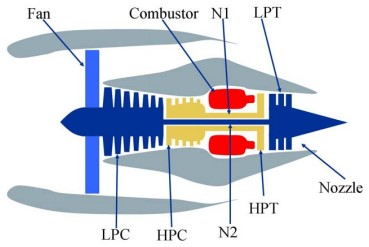
\includegraphics[width=.5\linewidth]{figures/c-mapss-engine-diagram.jpg}
    \caption{Simplified diagram of engine simulated in C-MAPSS \cite{Saxena2008}}
    \label{figure:c-mapss-engine-diagram}
\end{figure}

Table \ref{table:c-mapss-sensors} shows different variables, the output of the simulation and their units.

\begin{table}
    \centering
    \begin{tabular}{l|l|l}
        \hline
        \textbf{Symbol} & \textbf{Description} & \textbf{Units}\\
        \hline
        \textbf{T2} & Total temperature at fan inlet & R \\
        \textbf{T24} & Total temperature at LPC outlet & R \\
        \textbf{T30} & Total temperature at HPC outlet & R  \\
        \textbf{T50} &Total temperature at LPT & R\\
        \textbf{P2} & Pressure at fan inlet& psia\\
        \textbf{P15}& Total pressure in bypass-duct& psia\\
        \textbf{P30}& Total pressure at HPC outlet& psia\\
        \textbf{Nf}& Physical fan speed& rpm\\
        \textbf{Nc} & Physical core speed &rpm\\
        \textbf{epr}& Engine pressure ratio (P50/P2)& --\\
        \textbf{Ps30}& Static pressure at HPC outlet& psia\\
        \textbf{phi}& Ratio of fuel flow to Ps30& pps/psi\\
        \textbf{NRf}& Corrected fan speed &rpm\\
        \textbf{NRc}& Corrected core speed& rpm\\
        \textbf{BPR}& Bypass Ratio& --\\
        \textbf{farB}& Burner fuel-air ratio &--\\
        \textbf{htBleed}& Bleed Enthalpy &-- \\
        \textbf{Nf\_dmd} &Demanded fan speed& rpm\\
        \textbf{PCNfR\_dmd}& Demanded corrected fan speed &rpm\\
        \textbf{W31} & HPT coolant bleed & lbm/s \\
        \textbf{W32} & LPT coolant bleed & lbm/ \\
        \hline
    \end{tabular}
    \caption{C-MAPSS outputs to measure system response.}
    \label{table:c-mapss-sensors}
\end{table}


\section{Visualization of equipment degredation development using Principal Component Analysis}
Principal Component Analysis is a dimsneionality reduction technique, it was described in \ref{section:dimensionality-reduction}. In this section, PCA will be used to reduce the dimension of sensors data from C-MAPSS dataset for the purpose of visualization, if condition monitoring data is explicitly indicative of the equipment health state, visualization of principal components can show apparent visual degradation patterns.

\begin{figure}[H]
    \centering
    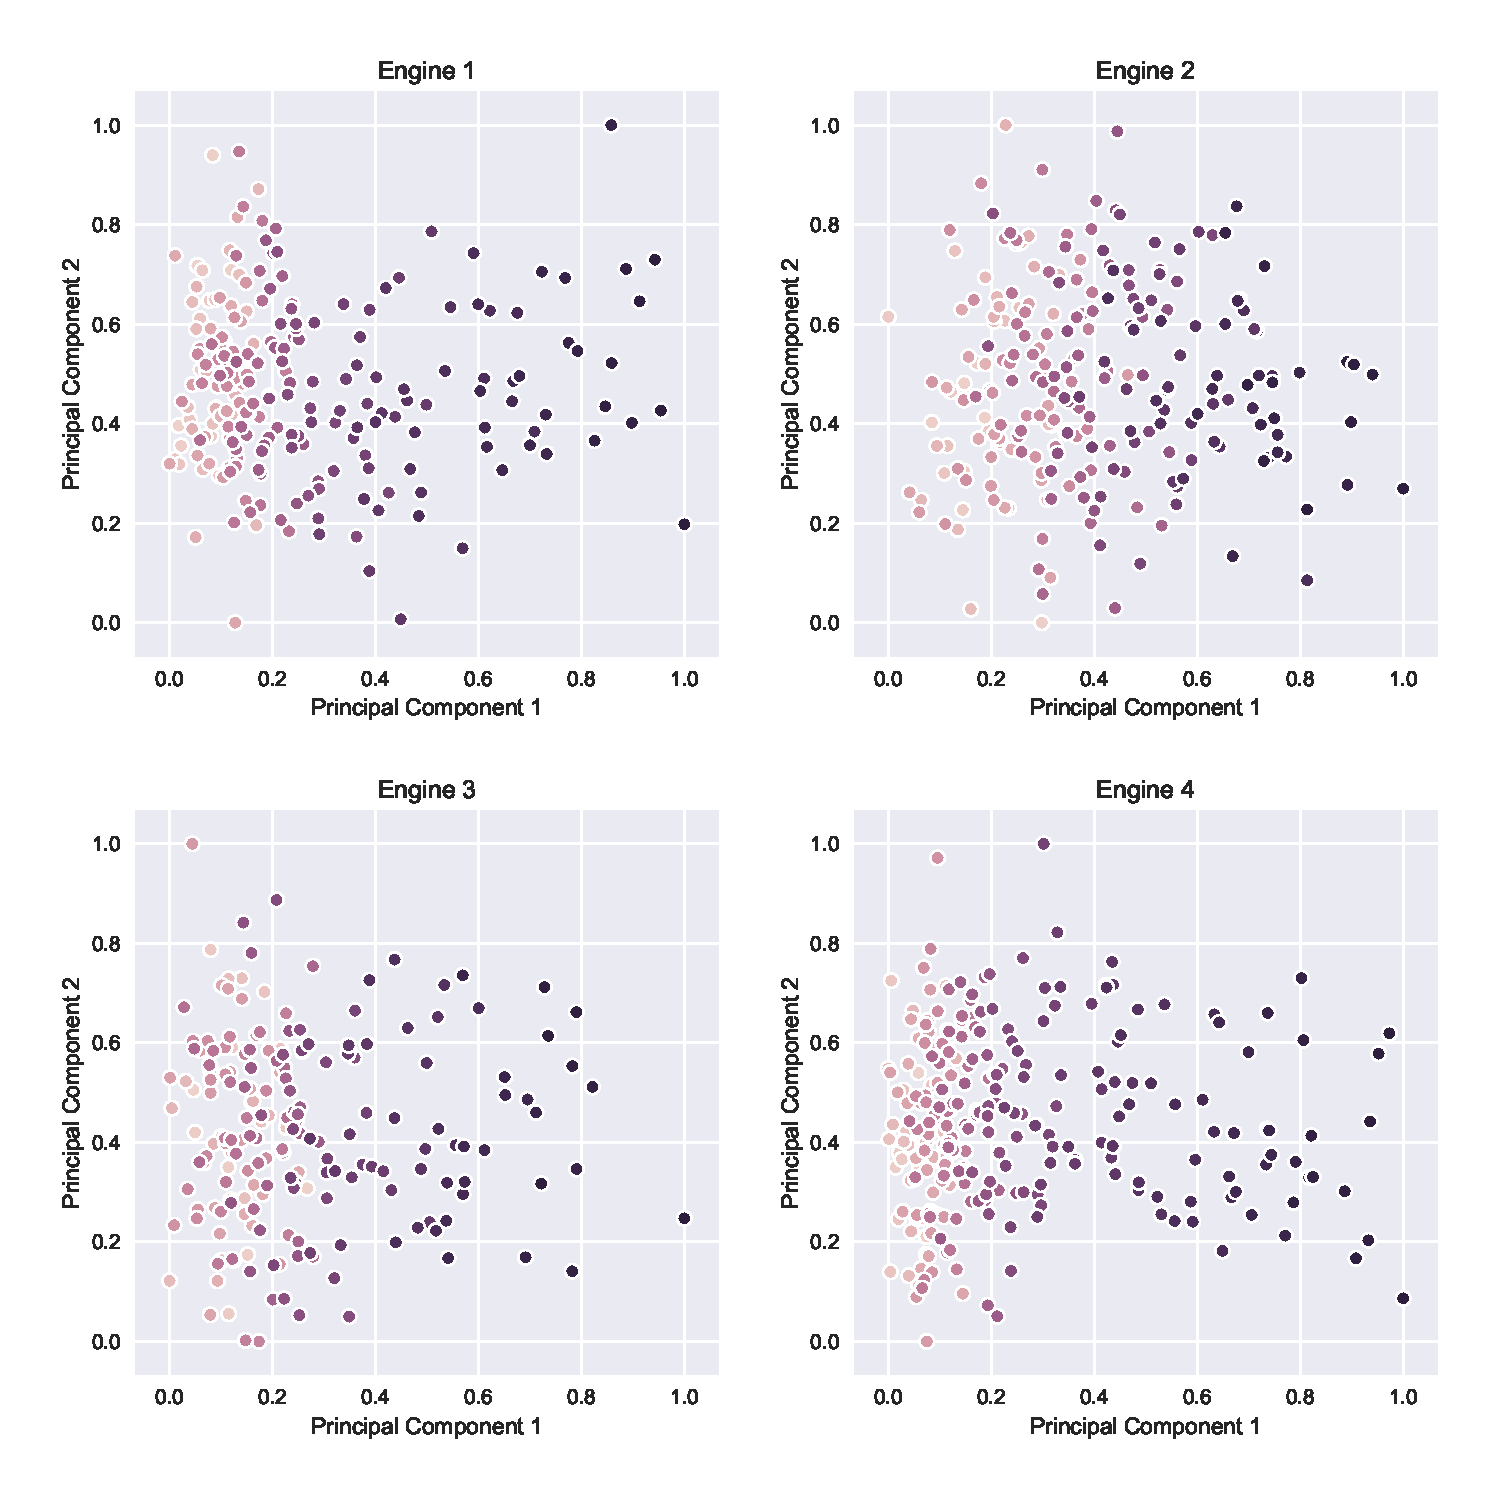
\includegraphics[width=\linewidth]{figures/plots/pc-degradation.pdf}
    \caption{Visualization of equipment health degredation development (lighter to darker colors) of different engines from C-MAPSS dataset by using Principal Component Analysis (PCA) for condition monitoring data dimensionality reduction.}
    \label{fig:pca-degradation}
\end{figure}

An apparent 

\section{Health state classification using neural networks}

\section{Conclusion}
